\talk{}{30}{%
\vspace{3mm}{\fontsize{25}{30}\selectfont\bfseries Area Optimization\\[1mm]After Technology Mapping}\par\vspace{6mm}{\fontsize{16}{20}\selectfont\color{Teal}Under a fixed delay bound}\par\vspace{8mm}{\large Shared logic, local rewriting, and reusable timing profiles}
}{各位老师、同学，大家好。今天我介绍工艺映射之后的面积优化。我们从已经映射成标准单元的网表出发，希望继续减少面积，同时保证最坏输出延迟不超过初始值。报告主要围绕三个问题展开：怎样产生更有效的候选结构，怎样正确计算共享逻辑的实际代价，以及怎样在有限时间内完成搜索。接下来先说明问题，再介绍方法和实验。}

\talk{Why optimize after mapping?}{60}{%
\begin{columns}[T]\column{.47\textwidth}\lead{Logic representation}\begin{itemize}\item AND-inverter graph (AIG)\item Node count and logic depth\end{itemize}\column{.47\textwidth}\lead{Mapped implementation}\begin{itemize}\item Standard-cell area and pin delays\item Shared cells and explicit inversions\end{itemize}\end{columns}\vspace{4mm}\[\text{Fewer AIG nodes}\;\not\Rightarrow\;\text{smaller standard-cell area}\]\vspace{2mm}A local rewrite saves area only when its old cells become removable.\src{Related work: [1] post-mapping optimization, [2] technology mapping and graph optimization.}
}{先看为什么工艺映射之后仍然值得优化。传统流程通常先减少 AIG 的节点数，再把逻辑图映射成标准单元。但是，AIG 节点数和实际单元面积并不是同一个目标。同样数量的与节点，可以对应不同的复合单元；不同的信号极性，还可能引入额外的反相器。另一个因素是共享：即使某个局部表达式变小，原来的逻辑如果仍被其他输出使用，就不能删除。因此，局部表达式的节省不一定转化成整个网表的节省。我们的出发点，就是直接保留映射后的结构，在真实的单元面积和引脚延迟模型下寻找替换。请注意屏幕上的关系：逻辑图更小，并不能直接推出标准单元面积更小。这也是后续所有估价和接受判断的依据。}

\talk{Problem formulation}{70}{%
\[\boxed{\min_N A(N)\quad\text{subject to}\quad D(N)\le D_0,\;N\equiv N_0}\]\vspace{2mm}\begin{align*}A(N)&=\sum_{v\in V_{\rm cell}(N)}a(v),&D_0&=D(N_0)\end{align*}\begin{itemize}\item $N_0$: initial mapped netlist. Keep $D_0$ fixed across rounds\item Minimize area first. Use delay to break area ties\item Allow local slack consumption within the global bound\end{itemize}\src{Area: $\mu\mathrm m^2$. Delay: ps, using library pin delays. Physical load and slew are outside this model.}
}{这一页给出我们真正求解的目标。面积是目标，延迟是约束，功能等价是必须满足的条件。式子中的 N 零是初始映射网表，D 零就是它的最坏输出延迟。我们首先保存这个值，之后无论执行多少轮，都使用同一个上界。如果某一轮把延迟降低了，下一轮也不会把这个更小的值强制设为新的上界，因为那可能阻止后续利用时序余量换取面积。另一方面，也绝不会把上界放宽到比原始网表更慢。具体比较时，先比较面积，面积相同时再选择延迟更小的结果。这里还有一个范围需要说明：延迟通过库中各输入引脚的延迟传播得到，没有引入布局布线之后的负载和转换时间。因此，后面说延迟不恶化，都是指这个明确的模型，而不是物理签核结果。}

\talk{Design questions}{30}{%
\begin{description}\item[Structure] Which equivalent implementations expose useful sharing?\vspace{4mm}\item[Cost] What area and delay will a replacement have in the live netlist?\vspace{4mm}\item[Search] How much candidate construction is affordable?\end{description}\vspace{4mm}\take{Method: 16 min \qquad Experiments: 9 min \qquad Discussion: 2 min}
}{围绕这个目标，方法需要回答三个问题。第一个是结构：怎样找到更容易共享、或者更适合库单元的等价实现？第二个是成本：把候选放回当前网表以后，到底新增哪些门、保留哪些旧门，延迟是否可行？第三个是搜索：怎样在有限时间内构建足够有用的候选？下面先用约十六分钟介绍方法，再用九分钟看实验，最后讨论目前的边界。}

\talk{Two optimization scopes}{80}{%
\begin{columns}[T]\column{.46\textwidth}\lead{Across roots}\vspace{2mm}\par Compose AO21 chain blocks.\par\vspace{3mm}Share factors and segments.\par\vspace{3mm}Evaluate one joint transaction.\column{.48\textwidth}\lead{Within one root}\vspace{2mm}\par Enumerate structural cuts.\par\vspace{3mm}Generate and price covers.\par\vspace{3mm}Use reverse topological order.\end{columns}\vspace{6mm}\take{Common guard: rebuilt area and the original delay bound}\src{A round starts from a checkpoint. Whole-window synthesis and unmap/remap exploration are disabled.}
}{从作用域来看，一轮优化有两个阶段。左边是跨根变换，先识别 AO21 链，把相邻步骤组合成块，再寻找多个根之间可以共享的因子和片段。由于共享会改变多个根的成本，我们把所有提案作为一个事务联合评估。右边是单根变换，按逆拓扑顺序访问节点，枚举结构 cut，为每个局部函数生成标准单元有向无环图，再根据当前网表的成本和时序选择替换。两个阶段的作用域不同，但接受原则一致：最终都要重建网表，检查面积和原始延迟上界。一轮开始时保存备份，检查失败就恢复。这里也明确当前实验的边界：整窗口综合和展开后重映射探索都关闭。因此，后面的收益应当归因于这两个明确的优化作用域。下面先看跨根阶段所用的精确变换。}

\talk{AO21 chain composition}{90}{%
An AO21 step represents $F_i(z)=(p_i\wedge z)\vee q_i$.\vspace{3mm}\begin{align*}F_1(F_2(z))&=p_1\wedge(p_2\wedge z\vee q_2)\vee q_1\\[2mm]&=\underbrace{(p_1\wedge p_2)}_{P}\wedge z\;\vee\;\underbrace{(q_1\vee p_1\wedge q_2)}_{Q}\end{align*}\vspace{2mm}\[\color{Teal}(P,Q)\circ(p,q)=(P\wedge p,\;Q\vee P\wedge q)\]\src{Exact Boolean identity, including dependent coefficient signals. Current configuration: two-step blocks, minimum chain length six.}
}{我们先看链结构为什么可以精确变换。一个 AO21 单元可以写成第一行的形式：p 和输入 z 相与，再与 q 相或。现在把第二个单元的输出代入第一个单元。展开以后，跟 z 相乘的系数变成 p 一与 p 二，而不含 z 的部分变成 q 一，或上 p 一与 q 二。这样，一段两级链又可以表示成同样的一对系数。屏幕下方的方框就是这个组合规则。这里有一个重要细节：它只使用布尔代数恒等式，没有假设这些系数信号相互独立；即使它们之间有逻辑依赖，变换也成立。实现中采用两步链块，只有入口链长度至少为六时才触发。我们并不是把所有链一概完全展开，而是在有限块内组合和平衡，以控制候选规模。理解这一点以后，就可以继续问：多个根之间，是否会出现相同的组合系数？这就引出了下一页的共享。}

\talk{Sharing changes the unit of evaluation}{70}{%
\begin{align*}y_r&=\color{Teal}P\color{Navy}\wedge z_r\vee Q_r\\[2mm]y_s&=\color{Teal}P\color{Navy}\wedge z_s\vee Q_s\end{align*}\begin{center}$P=p_1\wedge p_2$ is built once for both roots.\end{center}\vspace{2mm}\begin{itemize}\item Product memo: sorted, unique factors\item Segment memo: ordered coefficient pairs\item Rebuild the joint proposal to count all surviving cells\end{itemize}\take{Accept the transaction only when $A_{\rm new}<A_{\rm old}$ and $D\le D_0$}
}{现在假设两个根都需要同一个乘积 P，只是各自的数据输入和剩余项不同。那么，这个乘积可以只构建一次，同时供两个根使用。为了识别这种机会，我们保留两种记录。乘积记录的键，是经过排序和去重的因子信号，因为与运算不依赖排列顺序。链片段记录则保留系数对的原始顺序，因为组合方向会影响结果。更关键的是，不能对两个根分别估价，再简单地把节省相加。共享会让新门只计一次，也会让某些旧门继续存活。实现因此把这些提案作为一个事务共同构建，之后重建网表，统计真正存活的单元。只有总面积严格下降，而且最坏延迟仍满足初始上界，事务才会提交。这种评估方式既避免高估收益，也能发现单独替换不划算、联合共享后才有收益的结构。}

\talk{Local rewriting on structural cuts}{70}{%
\[\mathcal C=(x,L),\qquad |L|\le6\]\begin{columns}[T]\column{.47\textwidth}\lead{Boundary}\begin{itemize}\item $x$: root to replace\item $L$: signals cutting every input-to-root path\item Current arrivals belong to leaf signals\end{itemize}\column{.47\textwidth}\lead{Function}\begin{itemize}\item Truth table over $L$\item Conservative care set\item A replacement agrees on care minterms\end{itemize}\end{columns}\vspace{3mm}\src{Care-window simulation identifies unreachable minterms. Cofactor candidates and e-graph search use the full function. The window itself is not synthesized.}
}{链级阶段之后，我们转到局部替换。一个 cut 包含根节点 x 和一组叶节点 L。这里的叶节点不一定是主输入，它们也可以是网表内部的信号，所以每个叶节点都带有真实的到达时间。叶集截断所有从主输入到根的路径以后，就可以把根表示成关于这些叶变量的布尔函数。当前最多六个叶输入，因此可以用紧凑真值表进行功能匹配。对于某些因重汇合关系而不可能出现的叶输入组合，如果能够保守地证明不可达，就可以把它们作为无关项，放宽匹配条件。但不能证明的组合仍然必须保持原功能，相关候选和 e-graph 也使用完整函数。这里的窗口只用于计算 care 信息，不会被整体重新综合。换句话说，我们利用的是输入组合的可达性信息，替换的作用域仍由具体 cut 决定。}

\talk{Complementary candidate sources}{75}{%
\tblhead\begin{tabular}{@{}lP{7.8cm}@{}}\toprule Generator & Candidate structure\\\midrule L1: single cell & Function matching with phases and pin assignments\\[3mm]L2: database & Pre-mapped multi-cell directed acyclic graphs (DAGs)\\[3mm]L3: synthesis & Factoring, disjoint-support decomposition, and cofactors\\[3mm]L4: e-graph & Equivalent expressions with library-cell covers\\\bottomrule\end{tabular}\par\vspace{3mm}L1--L3 compete first. L4 is a fallback on the MFFC boundary cut.\src{MFFC: maximum fanout-free cone. L4 triggers only after no L1--L3 proposal passes the acceptance filters on that cut.}
}{我们使用四类候选来源。第一类是单单元匹配：通过功能、极性和输入置换，检查是否能直接用一个库单元替换。它很快，但是表达能力有限。第二类是预映射数据库，能够提供多个单元构成的小型有向无环图，但只能覆盖已经存储的函数和条目。第三类从布尔结构出发综合，包括积之和分解、可分解结构，以及后面重点介绍的 Shannon 和 Davio 展开。第四类是 e-graph，在等价表达式空间里保留多个结构，再提取库单元覆盖。四类生成器解决的是不同的覆盖问题，不能简单地认为只增加某一种搜索器的预算就足够了。与此同时，候选生成和候选估价是两个独立问题。即使产生了一个好结构，如果没有正确考虑外部共享或反相复用，最后仍可能把它错误地丢掉。}

\talk{Cofactor decompositions}{100}{%
For a pivot $\ell$, define $f_b=f|_{\ell=b}$ and $\Delta_\ell=f_0\oplus f_1$.\vspace{3mm}\begin{align*}f&=(\ell\wedge f_1)\vee(\neg\ell\wedge f_0)&&\text{Shannon}\\[3mm]f&=f_0\oplus(\ell\wedge\Delta_\ell)&&\text{Positive Davio}\\[3mm]f&=f_1\oplus(\neg\ell\wedge\Delta_\ell)&&\text{Negative Davio}\end{align*}\vspace{2mm}\take{Equivalent functions can produce different standard-cell covers}\src{Each form is factored, mapped, and verified independently on the complete cut truth table.}
}{这一页我们稍微放慢一点。先选择一个叶变量作为展开变量，把它取零和取一时的函数分别记为 f 零和 f 一，再定义它们的异或差，记为德尔塔。第一行是 Shannon 展开，也就是一个选择器：变量为一时选择 f 一，为零时选择 f 零。第二行是正 Davio，以 f 零为基础，只在展开变量为一时加入差分项。第三行是负 Davio，以 f 一为基础，在展开变量为零时加入差分项。三个公式实现同一个函数，但并不一定映射成同样的单元网络。例如，某种展开可能暴露可共享的子项，也可能允许一个信号绑定到复合单元的多个引脚。实现时，我们分别对余因子和差分项做积之和因式分解，构造 AIG，再独立映射和验证。因此，这里增加的不是几个形式上不同的公式，而是更多可能具有不同实际成本的候选结构。当然，如果对每个变量、每个家族都构建一遍，开销会很大，所以下一页介绍如何限制展开预算。}

\talk{Pivot selection under a search budget}{65}{%
Let $s(g)$ denote the number of support variables in $g$.\par\vspace{3mm}\tblhead\begin{tabular}{@{}lcl@{}}\toprule Family & Score to minimize & Retained pivots\\\midrule Shannon & $s(f_0)+s(f_1)$ & 2\\[2mm]Positive Davio & $s(f_0)+s(\Delta_\ell)$ & 2\\[2mm]Negative Davio & $s(f_1)+s(\Delta_\ell)$ & 2\\\bottomrule\end{tabular}\par\vspace{3mm}\begin{itemize}\item Resolve ties by leaf order, then process retained pivots in original order\item Check timing after mapping\end{itemize}\src{Support size is a heuristic. The cap can omit useful covers. The all-pivot ablation measures that tradeoff.}
}{这里用一个计算成本较低的结构特征来筛选展开变量，也就是函数的支持变量数。直观上，如果某次展开得到的两个部分只依赖较少变量，它们往往更容易产生紧凑结构。三个家族分别使用屏幕上的评分，并且分别保留两个变量，而不是所有家族共用两个名额。同分时按叶顺序处理；选出来之后，仍按原始顺序生成候选，避免额外改变处理轨迹。必须说明，这个分数既不是面积的精确预测，也不是时序可行性的证明。映射完成以后，还要使用真实叶到达时间检查延迟。因此，这项优化属于搜索覆盖的主动限制，可能漏掉更好的结构。后面的全变量消融会看到，取消限制确实还能减少一些面积，但也增加了耗时和超时。这是一个需要量化的质量与时间权衡。}

\talk{Bounded equality saturation}{65}{%
\lead{An e-class records equivalent expressions [3]}\vspace{4mm}\begin{enumerate}\item Expand the cut into an AIG with fixed leaf order\item Apply Boolean rewrites and library matching\item Initialize one area-oriented realization per e-class\item Widen the retained frontier within the remaining budget\end{enumerate}\vspace{3mm}\tblhead\begin{tabular}{@{}llll@{}}Iterations & e-nodes & Covers/class & Combined extraction budget\\\midrule 2 & 500 & up to 8 & 20,000 combinations / 4,000 visits\end{tabular}\src{Both extraction passes share one budget. Finite rules and frontiers give an incomplete candidate pool.}
}{接下来介绍第四类候选来源。我们先把 cut 内的单元展开成固定变量顺序的 AIG，再通过布尔重写和库匹配建立等价表达式。当前饱和过程限制为两次迭代和五百个节点。真正困难的部分通常是提取：一个类里有多个实现，而父节点要组合子节点的实现，组合数可能迅速增长。为此，我们先用较窄的面积导向前沿，为各个类建立基本覆盖，再在剩余预算中扩展到最多八个实现。两个阶段共享两万次组合和四千次访问上限，初始化并不是额外增加一份无限预算。它的作用，是避免早期几个类用完所有组合机会，而其他类连一个基本实现都没有。这里保留的前沿仍是有界近似，因此不能把它解释成整个等价空间的完整枚举。}

\talk{Timing profiles for reusable covers}{100}{%
\[T(H;\boldsymbol\tau)=\max_{i\in U_H}\bigl\{\tau(\ell_i)+p_i(H)\bigr\}\]\begin{center}{\small $p_i(H)$: input-to-root path delay. $U_H$: leaves used by $H$.}\end{center}\vspace{1mm}\begin{center}\tblhead\setlength{\tabcolsep}{10pt}\begin{tabular}{@{}lrrrr@{}}\toprule Cover & $p_0$ & $p_1$ & $T$ at $(0,0)$ & $T$ at $(20,0)$\\\midrule $H_1$ & 10 & 1 & 10 & \textcolor{Orange}{30}\\[2mm]$H_2$ & 1 & 10 & 10 & \textcolor{Teal}{21}\\\bottomrule\end{tabular}\end{center}\par\vspace{3mm}Store $\bigl(\widehat A(H),p_0,\ldots,p_{|L|-1}\bigr)$, then select using live arrivals.\src{Illustrative equal-area covers, delays in ps. Scalar zero-arrival delay loses this distinction. Bounded pruning uses the complete delay vector.}
}{这一页用一个小例子解释为什么要保存逐输入路径延迟。上面的公式表示，候选到达时间等于每个叶输入的当前到达时间，加上它到根的最长路径延迟，再取最大值。表中两个候选面积相同，延迟数字只是用于解释的例子，不是实验测量。第一个候选的两条路径分别是十和一，第二个是一和十。如果两个叶输入都在零时刻到达，两个候选的输出都是十，看起来没有区别。现在让第一个叶输入晚到二十，第二个输入仍在零时刻到达。第一个候选变成三十，第二个候选只有二十一。这说明，只存零到达时刻的一个标量，会丢失后续选择所需的信息。我们因此保存内在面积和完整路径向量，把当前到达时间留到现场使用时再代入。持久缓存命中后仍要重算现场成本，未命中才执行饱和与提取。有限前沿依然可能漏解，因此这里提供的是可复用候选池，而不是完整最优解集合。}

\talk{Area cost in the live netlist}{90}{%
\[u=\neg v\qquad\Longrightarrow\qquad\neg u=v\]\vspace{2mm}\[\widehat A_{\rm ctx}(H)=\underbrace{\sum_{v\in V_H^{\rm new}}a(v)}_{\text{new reachable cells}}+\underbrace{\sum_{v\in J_H\cap M}a(v)}_{\text{old cells retained by reuse}}\]\vspace{2mm}\[\Delta\widehat A(H)=\widehat A_{\rm ctx}(H)-\sum_{v\in M}a(v)\]\vspace{2mm}Resolve external phases before computing both area and timing.\src{$M$: removable old cells. $J_H$: reused old cells. Existing shared cells outside $M$ add no area. Reused signals must not depend on the replacement root.}
}{刚才保存的是候选的内在属性，现在还要把它放回实际网表中。最简单的例子是反相复用：如果已有 u 等于 v 的反相，那么再次对 u 取反，就直接得到 v，没有必要再新建一个反相器。还可以寻找已有的、确实通向输出的反相扇出。但复用并不意味着成本总是零。请看第二个公式，第一项统计实际新建而且最终可达的单元，第二项统计因为候选复用而保留下来的原可删除单元。第二项很容易漏掉：一个旧门本来可以随旧锥一起删除，现在因为被新候选引用而留下，就必须重新计入成本。相反，本来就被其他逻辑共享的旧门不能重复计价。最后还要检查环：被复用的信号不能依赖当前替换根，否则替换后会形成循环。完成相位解析以后，再在实际候选图上传播延迟，这样面积和时序才对应同一个可实现结构。}

\talk{Local feasibility and global acceptance}{75}{%
\begin{columns}[T]\column{.47\textwidth}\lead{Local selection}\vspace{2mm}\par Evaluate live leaf arrivals.\par\vspace{3mm}Require $T(H)\le R(x)$.\par\vspace{3mm}Rank by $\Delta\widehat A$, then arrival.\column{.47\textwidth}\lead{Global guard}\vspace{2mm}\par Check function and cycles.\par\vspace{3mm}Invalidate affected caches.\par\vspace{3mm}Rebuild and validate $(A,D)$.\end{columns}\vspace{5mm}\[R(o)=D_0,\qquad R(u)=\min_{(u,v,i)}\{R(v)-d_{v,i}-b_{v,i}d_{\rm inv}\}\]\src{$R$: required arrival time. $d_{v,i}$: pin delay. $b_{v,i}$: input-inversion indicator. A round rolls back if it violates $D_0$ or worsens the area-first objective.}
}{候选有了实际成本以后，还需要判断能不能接受。我们从输出端的固定延迟界限向后传播要求时间。公式里的引脚延迟和反相延迟，决定一个前驱最晚可以在什么时候到达。这使关键路径和非关键路径自然区别开来：关键部分的余量小，不能轻易增加延迟；非关键部分则可以在允许范围内消耗余量，争取更小面积。候选先满足根的要求时间，再按净面积增量排序。替换之前检查功能和循环依赖，替换之后使受影响的时序、cut 和查询缓存失效，因为旧信息可能已经不成立。局部检查只是选择依据。每一轮最后仍然重建整网表，重新统计面积和最坏输出延迟。只有全局目标没有变差才保留结果，否则回滚。这样，复杂的候选生成器共享同一套清晰的接受条件。}

\talk{Reusing work and restricting search}{65}{%
\begin{columns}[T]\column{.48\textwidth}\lead{Reuse computed results}\begin{itemize}\item Inverse-phase queries\item Truth-table simulation\item Mapped DAGs for identical AIG states\end{itemize}\vspace{2mm}{\small Recompute live cost and timing. Invalidate records when their context changes.}\column{.46\textwidth}\lead{Restrict candidate coverage}\begin{itemize}\item Two pivots per family\item Bounded saturation\item Limited extraction frontiers\end{itemize}\vspace{2mm}{\small Search limits can omit useful replacements.}\end{columns}\vspace{4mm}\take{Report solution quality, completion, and runtime separately}\src{Statistical deferrals are revisited. Only strict area bounds skip live pricing among generated covers.}
}{效率优化需要区分两种性质。前三项主要减少重复计算：已有反相器的查询结果可以复用，门功能和仿真工作区不必反复解析，相同的映射前 AIG 状态也可以复用已经得到的映射结构。但这些缓存都有有效条件，现场面积和时序仍然要重算。第四项不同，变量预算明确减少了候选覆盖。对于统计特征触发的延后操作，当前配置会补检，避免只因为一个启发式判断就永久放弃候选；只有严格的面积下界说明无法超过当前结果时，才跳过现场估价。这里不能笼统地把所有机制都称为无损加速。在有限时间预算和贪心替换顺序下，即使是减少重复计算，也可能间接影响最终轨迹。因此，实验必须分别报告 PPA、完成率和实际耗时。}

\talk{Experimental protocol}{70}{%
\tblhead\begin{tabular}{@{}lP{9.1cm}@{}}\toprule Item & Setting\\\midrule Designs & 16 fixed circuits with ASAP7 library models\\[2mm]mfs3 comparison & Same initial netlist, same 40-entry library ($\le6$ inputs)\\[2mm]Other experiments & Full 47-entry library, fixed original AIG inputs\\[2mm]Post-mapping budget & 1000 s for both tools\\[2mm]Disabled operations & Whole-window synthesis and unmap/remap exploration\\\bottomrule\end{tabular}\par\vspace{3mm}\src{The six-input restriction comes from the tested mfs3 implementation. Preprocessing, initial mapping, and combinational equivalence checking (CEC) are outside the post-mapping budget.}
}{下面进入实验，先明确公平性条件。所有实验使用固定的十六个电路和 ASAP7 库模型，原始 AIG 输入不变。与 ABC 的 mfs3 比较时，双方使用同一个初始映射网表，以及同一个至多六输入、包含四十项的子库。这个输入限制来自被测 mfs3 的实现。主实验和消融使用完整的四十七项库。双方后映射阶段都限制为一千秒，预处理、初始映射和组合等价检查不包含在这个预算中。整窗口综合与展开后重映射探索在所有相关实验中都关闭。因此，各配置之间改变的是后映射算法内部的机制，而不是输入和目标。冷、热缓存的详细区分会在运行时间页说明；这里先把输入、库和计时边界固定下来，接着看三部分实验各自能够支持什么结论。}

\talk{Evidence from three experiments}{45}{%
\tblhead\begin{tabular}{@{}P{3.1cm}P{3.7cm}P{5.0cm}@{}}\toprule Experiment & Starting netlist & Evidence sought\\\midrule Strong AIG optimization & $N_e$, round caps 1 and 6 & Remaining area opportunity\\[3mm]mfs3 (ABC [4]) & Same $N_i$, one round & Same-input tool comparison\\[3mm]Mechanism ablations & Same $N_e$, six-round cap & Quality and runtime tradeoffs\\\bottomrule\end{tabular}\par\vspace{3mm}$N_i$: direct mapping.\par $N_e$: mapping after high-effort AIG preprocessing.\src{ASPDAC'25 [1] has no available source implementation in this study. Its published costs are reconstructed separately, with different mapped inputs.}
}{三部分实验按照这张表的顺序展开。首先，充分优化 AIG，再映射得到固定起点，检验门级阶段还剩多少面积机会。第二部分与 ABC 的 mfs3 使用相同初始网表，观察工具之间的结果和可行性。第三部分从同一个充分预处理的起点逐项关闭机制，分析质量和运行时间的权衡。N i 表示直接映射的起点，N e 表示充分 AIG 预处理后再映射的起点，两者不能混用。至于 ASPDAC 二五年的文献比较，由于没有可运行源码，只能重建公开数值，不能保证初始映射相同。因此，它的结果单独讨论，不作为同输入算法优势的证明。下面先展示充分预处理后的主实验。}

\talk{Area gains after strong AIG optimization}{75}{%
\begin{columns}[T]\column{.60\textwidth}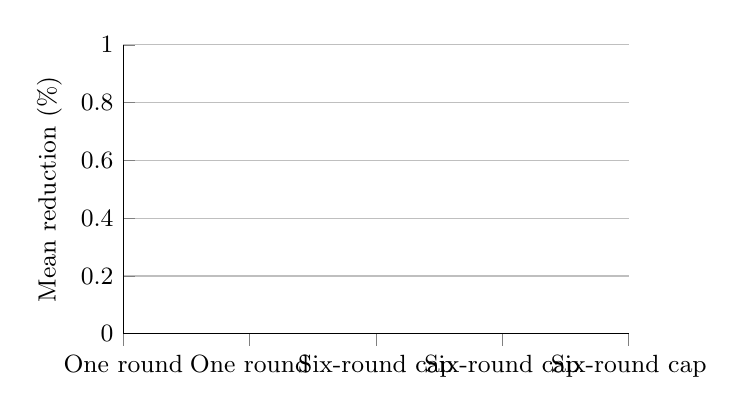
\begin{tikzpicture}\begin{axis}[width=8cm,height=5.25cm,ybar=8pt,bar width=12pt,symbolic x coords={One round,Six-round cap},xtick=data,ymin=0,ymax=9,ytick={0,2,4,6,8},ylabel={Mean reduction (\%)},ymajorgrids,axis lines*=left,enlarge x limits=.5,legend style={at={(.5,1.03)},anchor=south,legend columns=2,column sep=4pt,draw=none,font=\small},tick label style={font=\small},label style={font=\small},nodes near coords,nodes near coords style={font=\scriptsize,/pgf/number format/fixed,/pgf/number format/precision=2,/pgf/number format/fixed zerofill},every axis plot/.append style={draw=none}]\addplot[fill=Teal,area legend] coordinates {(One round,\OneArea) (Six-round cap,\MainArea)};\addlegendentry{Area}\addplot[fill=Orange,area legend] coordinates {(One round,\OneDelay) (Six-round cap,\MainDelay)};\addlegendentry{Delay}\end{axis}\end{tikzpicture}\column{.35\textwidth}\vspace{5mm}\lead{16 of 16}\par Smaller area, with $D\le D_0$.\vspace{6mm}\par\lead{3.59\%}\par Mean area reduction excluding arbiter.\end{columns}\src{Arithmetic mean of per-circuit percentage reductions. Caps 1 and 6 are independent runs. Cold and warm modes yield identical PPA.}
}{先看充分优化 AIG 之后，还能不能继续减少面积。图中每组是一个独立设置，左边只执行一轮，右边最多六轮。面积和延迟分别用两种颜色表示。单轮平均面积下降约百分之五点零四，延迟下降约百分之四点九零；六轮上限下，分别下降约百分之七点一一和七点四三。这里采用逐电路下降比例的算术平均，不是先把所有面积加起来再计算比例。十六个电路全部减少了面积，而且延迟都不超过初始上界。由于 arbiter 的收益较大，我们还单独检查了排除它的情况：其余十五个电路平均面积仍下降百分之三点五九。冷、热模式在这组实验中得到相同 PPA，所以后面主要通过运行时间体现缓存差异。这个结果说明，充分的逻辑优化以后，映射后的实现中仍有可恢复的面积空间。}

\talk{arbiter: a structural case study}{60}{%
\begin{columns}[T]\column{.52\textwidth}\tblhead\begin{tabular}{@{}lrr@{}}\toprule & Initial & Optimized\\\midrule Area ($\mu\mathrm m^2$) & 557.72 & \textcolor{Teal}{223.64}\\[2mm]Delay (ps) & 999.87 & \textcolor{Teal}{261.39}\\\bottomrule\end{tabular}\column{.42\textwidth}\lead{Same original input}\vspace{3mm}\par Chain composition exposes repeated factors across roots.\end{columns}\vspace{6mm}\[\underbrace{557.72-223.64}_{\text{area reduction}}=334.08\;\mu\mathrm m^2\]\src{Removing chain composition or cross-root sharing gives a summed area penalty of $+334.08$ in the ablations. Mechanism effects can interact.}
}{arbiter 的结果最突出。面积从五百五十七点七二降到二百二十三点六四，延迟从九百九十九点八七降到二百六十一点三九。这里始终保持原始起点不变，收益来自链级组合和跨根共享，而不是加强映射前的综合。消融也支持这个解释：去掉链组合，或者去掉跨根记录，都会丢掉三百三十四点零八的累计面积收益。不过，我们不能只用这个电路来说明整个方法。把 arbiter 排除以后，其余十五个电路的平均面积仍然下降约百分之三点五九。所以，链结构带来一个很大的代表性收益，而局部候选和估价机制在其他电路上也有作用。接下来再看更严格的同输入工具比较。}

\talk{Same-input comparison with mfs3}{90}{%
\begin{columns}[T]\column{.56\textwidth}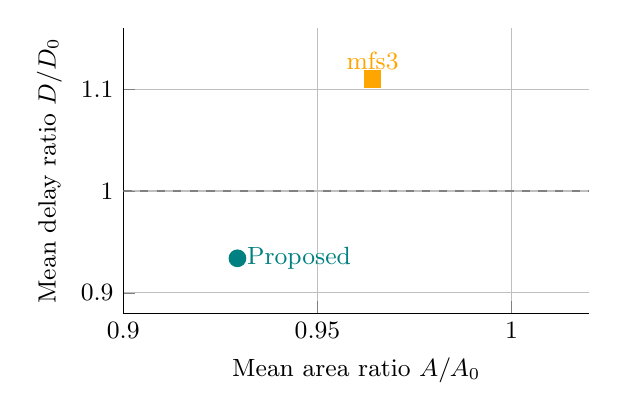
\begin{tikzpicture}\begin{axis}[width=7.5cm,height=5.2cm,xmin=.90,xmax=1.02,ymin=.88,ymax=1.16,xtick={.90,.95,1},ytick={.9,1,1.1},xlabel={Mean area ratio $A/A_0$},ylabel={Mean delay ratio $D/D_0$},axis lines*=left,grid=major,tick label style={font=\small},label style={font=\small}]\addplot[gray,dashed] coordinates {(.90,1)(1.02,1)};\addplot[only marks,mark=square*,mark size=3pt,Orange] coordinates {(.9642,1.1102)} node[above,font=\small]{mfs3};\addplot[only marks,mark=*,mark size=3pt,Teal] coordinates {(.9294,.9339)} node[right,font=\small]{Proposed};\end{axis}\end{tikzpicture}\column{.40\textwidth}\vspace{2mm}\lead{Completion}\par ABC: 13/16\par Proposed: 16/16\vspace{4mm}\lead{Delay violations}\par ABC: 7 completed cases\par Proposed: 0\par\vspace{4mm}{\small Raw area: 7 wins, 6 losses versus ABC on completed pairs.}\end{columns}\src{Points are means over the 13 ABC-completed pairs, using each tool's native imported baseline. mfs3 -a does not enforce $D_0$. Dashed line: unit mean delay ratio.}
}{这张图把同输入对照的平均面积和延迟放在两个坐标轴上。越向左，平均面积比例越小；越向下，平均延迟比例越小。两个点都只根据 ABC 正常完成的十三个电路计算，并按各工具导入后的原生初始成本归一化。ABC 的面积比例是零点九六四二，延迟比例是一点一一零二；我们分别是零点九二九四和零点九三三九。虚线标出单位延迟比例，但均值在线下不代表逐电路都满足约束，因此右边另列违例数：ABC 有七个完成结果超过初始延迟，我们是零个。完整样本中，ABC 完成十三个，我们完成十六个。还要保留一个限制：逐项比较原始输出面积，我们七胜六负，并非每个电路都占优。由于 mfs3 的面积选项不强制原始延迟界限，这张图支持的是当前协议下的整体质量与可行性结论，而不是所有目标设置下的绝对优越性。}

\talk{Completion and cache-dependent runtime}{65}{%
\begin{columns}[T]\column{.56\textwidth}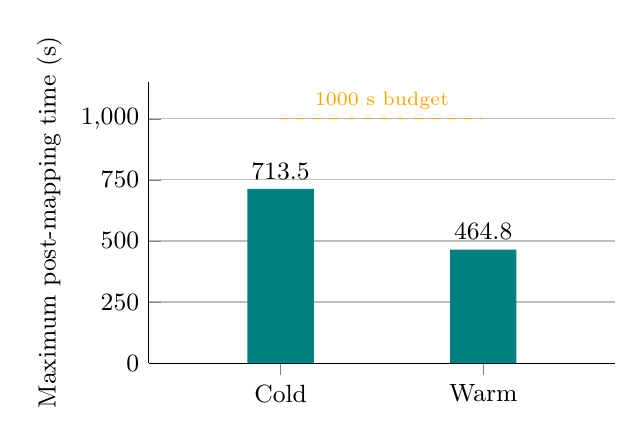
\begin{tikzpicture}\begin{axis}[width=7.5cm,height=5.15cm,ybar,bar width=24pt,symbolic x coords={Cold,Warm},xtick=data,ymin=0,ymax=1150,ytick={0,250,500,750,1000},ylabel={Maximum post-mapping time (s)},ymajorgrids,axis lines*=left,enlarge x limits=.65,tick label style={font=\small},label style={font=\small},nodes near coords,nodes near coords style={font=\small}]\addplot[fill=Teal,draw=none] coordinates {(Cold,713.5)(Warm,464.8)};\addplot[Orange,dashed,sharp plot,update limits=false,nodes near coords={}] coordinates {(Cold,1000)(Warm,1000)} node[pos=.5,above,font=\scriptsize]{1000 s budget};\end{axis}\end{tikzpicture}\column{.40\textwidth}\vspace{2mm}\lead{128/128 completed}\par Full configuration only.\par\vspace{3mm}\tblhead\begin{tabular}{@{}lr@{}}\toprule Paired mean (s) & Time\\\midrule Proposed, cold & 75.0\\Proposed, warm & 27.8\\ABC & 26.4\\\bottomrule\end{tabular}\par\vspace{2mm}{\small Cold: empty profile pool. Warm: corresponding cold pool.}\end{columns}\src{Deadline: 1000 s. 64 runs per mode across four full-configuration settings. Native caches restart. OS caches remain. Shared-host, single-run timing. Controls have 7 TOs.}
}{运行时间这里分成两个口径。左图表示完整配置在每种缓存模式下最长的一次后映射时间，冷运行约七百一十三点五秒，热运行约四百六十四点八秒，均低于一千秒截止。右侧的一百二十八次完成，是四种完整配置设置、十六个电路、两个缓存模式的总计，并不是一百二十八个不同电路。右边小表则只看与 ABC 正常完成的十三个电路配对的平均时间，冷缓存七十五秒，热缓存二十七点八秒，ABC 二十六点四秒。冷运行使用私有空持久池，热运行只加载对应冷池；原生缓存重启，操作系统缓存不清除。由于是共享主机上的单次测量，不能据此宣称普遍加速。更准确的结论是，完整配置在这批运行中都完成了，而关闭部分机制的控制仍有七个超时。}

\talk{Area penalties from removing mechanisms}{65}{%
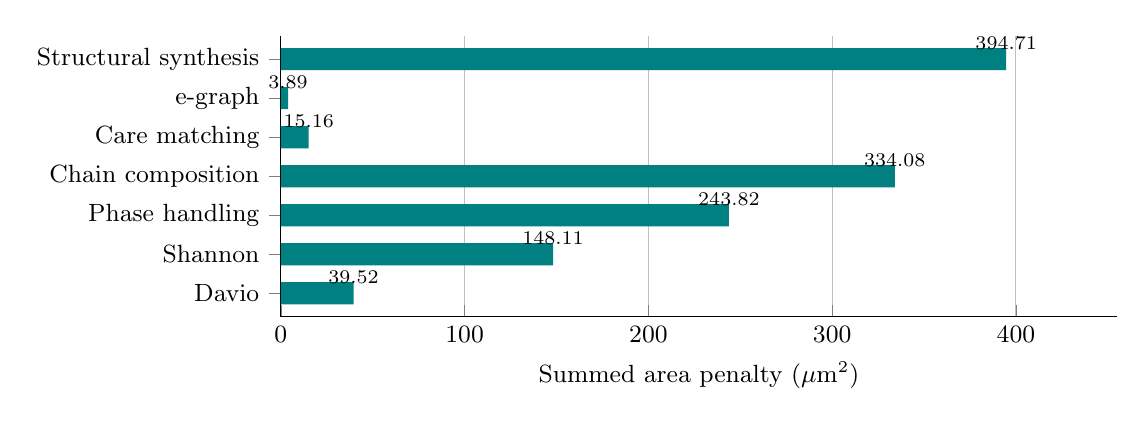
\begin{tikzpicture}\begin{axis}[width=12.2cm,height=5.15cm,xbar,bar width=8pt,xmin=0,xmax=455,xtick={0,100,200,300,400},xlabel={Summed area penalty ($\mu\mathrm m^2$)},ytick={1,2,3,4,5,6,7},yticklabels={Davio,Shannon,Phase handling,Chain composition,Care matching,e-graph,Structural synthesis},ymin=.4,ymax=7.6,axis lines*=left,xmajorgrids,tick label style={font=\small},label style={font=\small},nodes near coords,nodes near coords align={horizontal},nodes near coords style={font=\scriptsize},point meta=explicit symbolic]\addplot[fill=Teal,draw=none] coordinates {(39.52,1)[39.52](148.11,2)[148.11](243.82,3)[243.82](334.08,4)[334.08](15.16,5)[15.16](3.89,6)[3.89](394.71,7)[394.71]};\end{axis}\end{tikzpicture}\src{$\Sigma\Delta A=\sum_d(A_{d,\rm disabled}-A_{d,\rm full})$. Same area penalties in cold and warm modes. All shown controls complete. Effects are not additive. Full runtime data are in the appendix.}
}{这里把主要结构机制的消融画成面积损失条形图。横轴是关闭机制以后，相对于完整配置的累计面积增加，数值越大，说明移除后的损失越明显。冷、热两组在这些行上的面积差相同，而且都正常完成，所以可以直接比较这组面积结果。结构综合和链组合的影响较大，物理相位处理也不可忽略。Shannon 与 Davio 分别带来不同的候选机会。care 匹配和 e-graph 的累计影响较小，但仍然能够影响具体电路的选择。这里的数值不是独立贡献，不能把条形长度相加：关闭一个机制会改变中间网表，进而改变后续 cut、共享条件和贪心轨迹。这些消融衡量的是，在当前完整方法背景下移除某一机制，会对最终结果产生什么后果。各控制的运行时间和完整结果保留在附录。}

\talk{Reuse and search coverage: different tradeoffs}{75}{%
\tblhead\begin{tabular}{@{}lrrr@{}}\toprule Control & $\Sigma\Delta A$ & Time/full & TOs\\\midrule No query reuse & +69.76 / +68.63 & 1.67 / 2.15 & 2 / 2\\[2mm]No table reuse & +0.00 / +0.00 & 1.02 / 1.02 & 0 / 0\\[2mm]All pivots & $-36.93$ / $-39.99$ & 1.28 / 1.55 & 1 / 1\\\bottomrule\end{tabular}\par\vspace{3mm}\begin{itemize}\item Query reuse: same PPA on 14 completed pairs\item Table reuse: same PPA on all 16 circuits\item All pivots: extra area savings, with mem\_ctrl timing out\end{itemize}\src{Pairs show cold / warm. Area differences in $\mu\mathrm m^2$. Query control also removes the level shortcut. Table control retains scalar cut memoization. Time includes TO budgets, so ratios are not equal-work speedups.}
}{最后三组消融把计算复用和搜索预算的区别表现得更清楚。关闭查询加速以后，div 和 sqrt 在冷、热两组都超时；其余十四个完成配对的面积和延迟没有改变。这里的控制同时关闭查询记录和层级快速否定，所以不能把全部开销只归因于一个哈希表。关闭真值表复用以后，十六个电路的 PPA 都不变，累计耗时增加约百分之二；公共的标量 cut 记录仍然保留。全变量控制则不同，它真的搜索了更多候选，冷、热分别额外减少三十六点九三和三十九点九九的累计面积，但 mem_ctrl 在两组都超时。这说明固定两个变量的预算确实损失了一部分面积机会。表中的时间比包含截止预算，不能视为完成同样工作量的纯加速比。下一步更值得研究的，是把预算优先分配给更可能有效的结构。}

\talk{Scope of the evidence}{60}{%
\tblhead\begin{tabular}{@{}P{5.7cm}P{6.3cm}@{}}\toprule Supported by these experiments & Remaining limitations\\\midrule Area gains at fixed initial delay & Library timing, without physical sign-off\\[3mm]Budget completion on the tested suite & Finite rules and frontiers can miss covers\\[3mm]Same-input mfs3 comparison & Different internal delay objectives\\[3mm]Cold/warm runtime observations & Shared host and no repeated-run statistics\\\bottomrule\end{tabular}\par\vspace{3mm}\src{ASPDAC'25 literature reconstruction: 14/16 smaller final areas, but different mapped inputs. This does not isolate a post-mapping algorithm advantage.}
}{在结束之前，我把结论的边界集中说明。首先，有限重写规则、有限前沿和变量上限都会漏解，当前方法没有完整最优性保证。其次，profile 与当前叶到达时间无关，只是支持跨查询复用，并不表示它已经包含所有外部共享条件。再次，ASPDAC 二五年的文献重建中，十六个电路有十四个最终面积更小，但起点不同，所以不能把差值全部归因于后映射算法。运行时间来自共享主机上的单次观察，延迟来自库模型，这两点也限制了结论的适用范围。基于这些结果，下一步可以考虑按结构特征分配候选预算，同时保留固定输入、固定时序界限和明确的接受规则，使收益与开销都能够复现和解释。}

\talk{Conclusions}{60}{%
\begin{enumerate}\item Mapped-cell structure retains area opportunities after AIG optimization\vspace{3mm}\item Cross-root sharing and local covers address different scopes\vspace{3mm}\item Reusable profiles require live timing and sharing evaluation\end{enumerate}\vspace{3mm}\lead{16/16 main circuits: smaller area, no delay regression}\vspace{5mm}\par\textbf{Open question}\par How should circuit structure determine the search budget?
}{最后总结三点。第一，充分的 AIG 优化之后，标准单元网表仍有进一步减少面积的空间。第二，链级共享和局部候选覆盖的是不同作用域，需要分别生成结构，再统一评估。第三，可复用 profile 保存结构属性，但每次使用时仍必须结合当前到达时间和共享关系重新判断。效率方面，计算复用减少重复工作，搜索预算则可能损失候选覆盖，必须同时报告质量和时间。当前实验中，十六个主实验电路都减少了面积，而且没有延迟退化；完整配置的一百二十八次运行均在预算内完成。接下来值得讨论的是，能否让电路结构决定每个 cut 的搜索预算，把更多时间留给真正可能产生收益的局部问题。我的报告到这里，谢谢大家，欢迎讨论。}

\appendix

\begin{frame}{Appendix: main results, 1/2}
\small\renewcommand{\arraystretch}{1.15}\setlength{\tabcolsep}{5pt}
\begin{tabular}{@{}lrrrrr@{}}\toprule Circuit & $A_0$ & $A$ & $D_0$ & $D$ & $t_c/t_w$ (s)\\\midrule
\MainRowsA
\bottomrule\end{tabular}
\src{Full library; six-round cap. Area in $\mu\mathrm m^2$, delay in ps; same initial netlists; identical cold/warm PPA.}
\note{这里给出主实验前八个电路的完整数据。左侧是初始面积和优化后面积，中间是对应延迟，右侧是冷、热运行时间。所有行使用完整库和相同起点，延迟都没有超过初始值。可以看到，arbiter 的结构性收益最明显，而其他电路的变化幅度并不一致。}
\end{frame}

\begin{frame}{Appendix: main results, 2/2}
\small\renewcommand{\arraystretch}{1.15}\setlength{\tabcolsep}{5pt}
\begin{tabular}{@{}lrrrrr@{}}\toprule Circuit & $A_0$ & $A$ & $D_0$ & $D$ & $t_c/t_w$ (s)\\\midrule
\MainRowsB
\bottomrule\end{tabular}
\src{Full library; six-round cap. Area in $\mu\mathrm m^2$, delay in ps; same initial netlists; identical cold/warm PPA.}
\note{这一页是其余八个电路。例如，tv80 的面积从三百四十点六一降到三百三十点八七；usb_phy 从二十二点五四降到二十一点三九。面积改善较小时，同样需要保留实际延迟和时间，避免只展示百分比而忽略优化开销。}
\end{frame}

\begin{frame}{Appendix: same-input ABC comparison, 1/2}
\small\renewcommand{\arraystretch}{1.15}\setlength{\tabcolsep}{4pt}
\begin{tabular}{@{}lrrrrrr@{}}\toprule & \multicolumn{3}{c}{ABC mfs3} & \multicolumn{3}{c}{Proposed method}\\
Circuit & $A/A_0$ & $D/D_0$ & $t$ (s) & $A/A_0$ & $D/D_0$ & $t_c/t_w$ (s)\\\midrule
\AbcRowsA
\bottomrule\end{tabular}
\src{Same $\le6$-input library and initial netlist. Native baseline normalization; $\dagger$: delay violation; TO: 1000 s. CEC excluded.}
\note{这里是同输入 ABC 比较的前半部分。所有比例都按各工具自己的原生初始成本归一化。带剑号的延迟表示超过原始上界，TO 表示达到一千秒截止。超时行仍然保留，不能从整体完成率中删除。}
\end{frame}

\begin{frame}{Appendix: same-input ABC comparison, 2/2}
\small\renewcommand{\arraystretch}{1.15}\setlength{\tabcolsep}{4pt}
\begin{tabular}{@{}lrrrrrr@{}}\toprule & \multicolumn{3}{c}{ABC mfs3} & \multicolumn{3}{c}{Proposed method}\\
Circuit & $A/A_0$ & $D/D_0$ & $t$ (s) & $A/A_0$ & $D/D_0$ & $t_c/t_w$ (s)\\\midrule
\AbcRowsB
\bottomrule\end{tabular}
\src{Same $\le6$-input library and initial netlist. Native baseline normalization; $\dagger$: delay violation; TO: 1000 s. CEC excluded.}
\note{这是同输入比较的后半部分。请注意，有些电路 ABC 的原始输出面积更小，但对应延迟也可能超过初始上界。因此，对照需要同时看面积、延迟可行性和完成情况，不能只按某一列判断。}
\end{frame}

\begin{frame}{Appendix: complete ablations, 1/2}
\small\renewcommand{\arraystretch}{1.05}\setlength{\tabcolsep}{7pt}
\begin{tabular}{@{}lrrr@{}}\toprule Control & $\Sigma\Delta A$ C/W & Time/full C/W & TOs C/W\\\midrule
\AblationRowsA
\bottomrule\end{tabular}
\src{C/W: cold/warm. Area difference in $\mu\mathrm m^2$, positive is worse. Verified timeout snapshots retain incomplete status.}
\note{这张表列出前十组完整消融。每一行只改变所列机制，其余配置和起点保持一致。面积差是相对于完整配置的累计变化，冷、热分别报告。它反映移除机制之后的整体后果，不是可以直接相加的独立贡献。}
\end{frame}

\begin{frame}{Appendix: complete ablations, 2/2}
\small\renewcommand{\arraystretch}{1.05}\setlength{\tabcolsep}{7pt}
\begin{tabular}{@{}lrrr@{}}\toprule Control & $\Sigma\Delta A$ C/W & Time/full C/W & TOs C/W\\\midrule
\AblationRowsB
\bottomrule\end{tabular}
\src{C/W: cold/warm. Area difference in $\mu\mathrm m^2$, positive is worse. Verified timeout snapshots retain incomplete status.}
\note{这里是剩余九组消融。查询复用和变量预算对预算内完成比较重要；真值表复用、精确 AIG 复用和只读库共享的影响较小。全变量控制有额外面积收益，但在两个缓存模式中都出现超时，体现了候选覆盖与时间之间的权衡。}
\end{frame}

\begin{frame}{Appendix: parameters and validation}
\begin{itemize}\item Cuts: $K=6$, 12 cuts per root; e-graph threshold $\theta=0$\item Care: 8-input reconvergent window; full care after 60 s; SAT off\item Database: three levels, area cap 0.50; native cache: 262144 entries\item Profiles: 2 iterations, 500 nodes, 8 covers, 20000 combinations, 4000 visits\item 2 pivots per family; SOP/DSD: $\ge4$ leaves; Shannon/Davio: $\ge3$\item Periodic legal snapshots; independent CEC and serialized PPA audit for TOs\item Shared host: up to 12 method jobs and 6 ABC jobs, one observation per case\end{itemize}
\note{这一页保留了复现所需的主要参数。cut 最多六个叶，每个根保留十二个 cut；e-graph 和提取都有明确的节点、组合和访问上限。达到截止的运行使用此前保存的合法网表，并独立检查等价性和实际成本，但仍然按未完成统计。}
\end{frame}
\begin{frame}{Appendix: references}
\small
\begin{enumerate}\item[{[1]}] A. Costamagna et al. \textit{Area-Oriented Optimization After Standard-Cell Mapping}. ASPDAC, 2025. DOI: 10.1145/3658617.3697722.
\item[{[2]}] A. Tempia Calvino et al. \textit{A Versatile Mapping Approach for Technology Mapping and Graph Optimization}. ASPDAC, 2022.
\item[{[3]}] M. Willsey et al. \textit{egg: Fast and Extensible Equality Saturation}. PACMPL/POPL, 2021.
\item[{[4]}] R. Brayton and A. Mishchenko. \textit{ABC: An Academic Industrial-Strength Verification Tool}. CAV, 2010.
\end{enumerate}
\vspace{2mm}Experimental data: fixed 16-circuit campaign. Main and ablation tables use the same admitted output records. Source hashes accompany the LaTeX data snapshot.
\note{这里列出相关工作，包括映射后面积优化、图优化与映射、等价饱和以及 ABC。今天展示的数字来自同一轮固定实验，完整的逐电路表格和数据来源随源码保留。如果有具体的结构或实验口径问题，可以回到相应附录继续讨论。}
\end{frame}
